\documentclass[10pt]{beamer}
\usetheme[background=light, progressbar=foot, titleformat=allcaps]{metropolis}

\usepackage[authoryear]{natbib}
\usepackage{relsize}
\usepackage{caption}
\usepackage{amsmath, amsfonts}
\usepackage{booktabs}
\usepackage{longtable}
\usepackage{array}
\usepackage{multirow}
\usepackage{float}
\usepackage{tabu}
\usepackage{threeparttable}
\usepackage{adjustbox}

\usepackage[T1]{fontenc}
\usepackage[scaled]{uarial}
\setbeamercolor{background canvas}{bg=white}
\renewcommand*\familydefault{\sfdefault}

\title{Debt, Growth, and Inequality}
\author{Anthony Eisenbarth \& Zhuo Chen}
\begin{document}
\begin{frame}[plain]
    \maketitle
\end{frame}
\begin{frame}{Introduction}
	
\begin{itemize}
	\item 
	In the aftermath of the Great Recession and the COVID-19 pandemic public debt levels have soared to unprecedented levels. The extraordinary high debt levels and seeming fragility of the global economy has brought public and academic debate to reconsider the long-run implications of fiscal spending. Modern arguments can be traced back to Buchannan (1958), Meade (1958), and Modigliani (1961), although the issue goes back as far as Adam Smith.
	\item The empirical relationship between public debt and economic growth in OECD and developing countries has been studied exhaustively.
	\item What has not been as extensively covered is the relationship between gross government debt, economic growth, and the distribution of income.
	\end{itemize}
\end{frame}

\begin{frame}{Data}
\begin{itemize}
	\item We construct a rich dataset combining data on gross government debt from the International Monetary Fund International Financial Statistics database, growth data from the World Development Indicators database maintained by the World Bank, and additional data from the Penn World Tables (10.0).
	\item For our response variable, we utilize the data provided by the Standardized World Income Inequality Database (Solt 2020), which is a comprehensive database for country-wide estimates of the Gini coefficient for 196 countries covering 1960 to the present.
	\item Since our analysis allows for slope heterogeneity across countries, we need a sufficient
	number of time periods to estimate country-specific coefficients. To this end, we include only countries in our sample for which we have at least 30 consecutive annual observations on debt, the Gini coefficient, and GDP. 
\end{itemize}
\end{frame}

\begin{frame}
	\begin{table}
		\caption{Included Countries}
		\centering
		\begin{adjustbox}{max width=\textwidth}
		\begin{tabular}{lrrrrr}
			\toprule
			Region & Upper Middle Income & High Income & Low Income & Lower Middle Income & Total\\
			\midrule
			Latin America \& Caribbean & 11 & 5 & 0 & 2 & 18\\
			East Asia \& Pacific & 4 & 5 & 0 & 1 & 10\\
			Europe \& Central Asia & 1 & 18 & 0 & 0 & 19\\
			Sub-Saharan Africa & 3 & 0 & 10 & 9 & 22\\
			South Asia & 0 & 0 & 0 & 5 & 5\\
			North America & 0 & 2 & 0 & 0 & 2\\
			Middle East \& North Africa & 0 & 0 & 0 & 6 & 6\\
			Total & 19 & 30 & 10 & 23 & 82\\
			\bottomrule
		\end{tabular}
		\end{adjustbox}
	\end{table}
	
\end{frame}


\begin{frame}{}
	\centering
			\begin{threeparttable}
				\tiny
				\caption{Income Classification of Countries}
				\begin{tabular}{llll}
					\toprule
					\textbf{High income} & \textbf{Low income} & \textbf{Lower middle income} & \textbf{Upper middle income} \\
					\midrule
					Australia & Burkina Faso & Bangladesh & Argentina \\
					Austria & Central African Republic & Bolivia & Brazil \\
					Belgium & Gambia & Cote d'Ivoire & Botswana \\
					Barbados & Madagascar & Algeria & China \\
					Canada & Mali & Egypt & Colombia \\
					Switzerland & Malawi & Ghana & Costa Rica \\
					Chile & Niger & Honduras & Ecuador \\
					Cyprus & Rwanda & India & Guatemala \\
					Germany & Sierra Leone & Iran & Indonesia \\
					Denmark & Uganda & Jordan & Jamaica \\
					Spain &  & Kenya & Mexico \\
					Finland &  & Sri Lanka & Mauritius \\
					France &  & Lesotho & Malaysia \\
					United Kingdom &  & Morocco & Peru \\
					Greece &  & Mauritania & Paraguay \\
					Ireland &  & Nigeria & El Salvador \\
					Italy &  & Nepal & Thailand \\
					Japan &  & Pakistan & Turkey \\
					South Korea &  & Philippines & South Africa \\
					Luxembourg &  & Senegal &  \\
					Netherlands &  & Tunisia &  \\
					Norway &  & Zambia &  \\
					New Zealand &  & Zimbabwe &  \\
					Panama &  &  &  \\
					Portugal &  &  &  \\
					Singapore &  &  &  \\
					Sweden &  &  &  \\
					Trinidad and Tobago &  &  &  \\
					Uruguay &  &  &  \\
					United States &  &  &  \\
					\bottomrule
				\end{tabular}
\end{threeparttable}
\end{frame}

\begin{frame}
	\begin{figure}
		\caption{Debt and Inequality}
		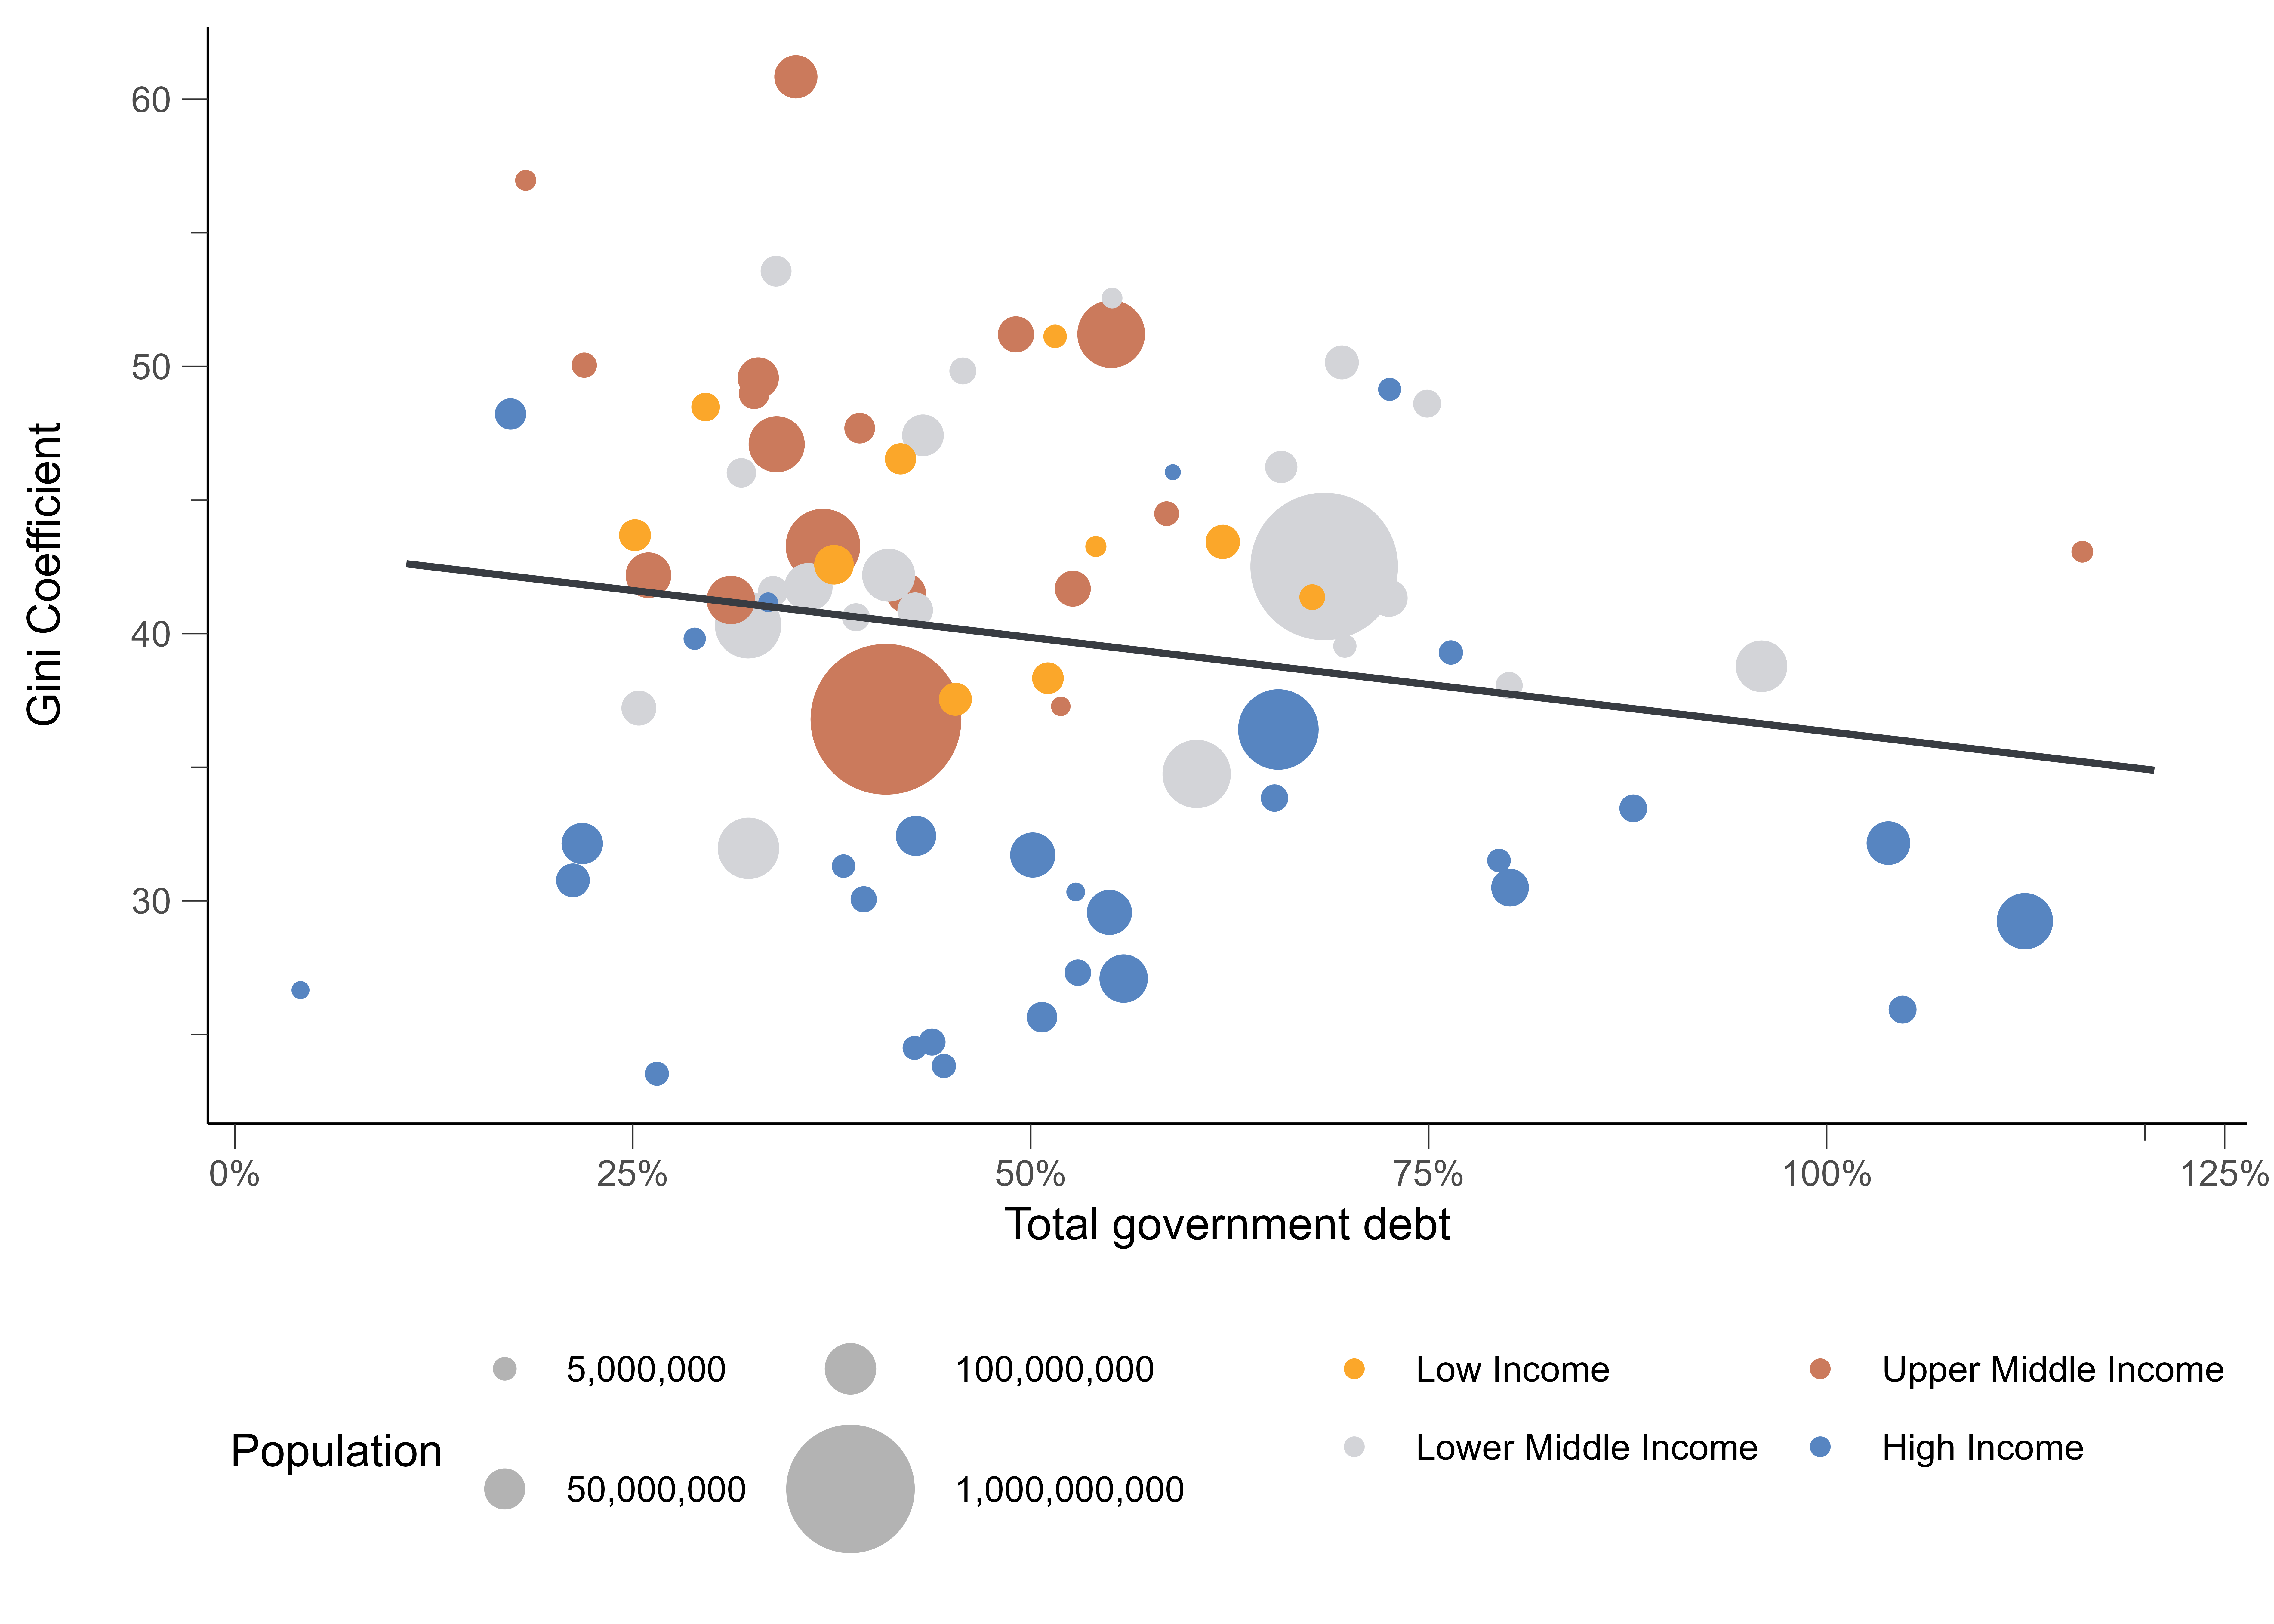
\includegraphics[width=\textwidth]{figure1.png}
	\end{figure}
	
\end{frame}

\begin{frame}{Methodology}
\begin{itemize}
\item Our sample restrictions provide us a dataset of 82 countries, with a time span of 1973 to 2019. 
	
\item 
We first consider the long-run effects of debt and output growth on the distribution of income using a traditional panel fixed-effects approach, in the following equation:
\begin{equation}
y_{it} = \alpha_{i} + \lambda_{t} + \gamma d_{it} + \mathbf{\beta}\mathbf{X}_{it} + u_{it}
\end{equation}
where $y_{it}$ is the log of the Gini coefficient and $\mathbf{x}_{it}$ a vector of exogenous variables including the the log of debt to GDP ratio $d_{it}$, and $g_{it}$ the growth rate. $\alpha_{i}$ and $\lambda_{t}$ are country and time specific fixed-effects. 
\end{itemize}

\end{frame}

\begin{frame}{Results}
	\begin{itemize}
		\item As a baseline, we fit a pooled model of all 82 countries together. Then we fit separate models based on the IMF income classifications.
		\item We also consider the interaction effect between the debt level and the growth rate.
		\item  By fitting these models to different income groups, we aim to uncover distinct patterns and relationships between income inequality and economic indicators across varying levels of economic development.
	\end{itemize}
\end{frame}

\begin{frame}
	\begin{center}
	\begin{threeparttable}[!htbp] \centering \footnotesize
		\caption{Regression Results} 
		\label{} 
		\begin{tabular}{@{\extracolsep{5pt}}lccccc} \toprule
			 & (1) & (2) & (3) & (4) & (5) \\
			\hline \\[-1.8ex] 
			Total debt & -0.004 & 0.002 & 0.043$^{**}$ & 0.010 & 0.063$^{**}$  \\ 
			& (0.045) & (0.081) & (0.025) & (0.031) & (0.031) \\ 
			& & & & & \\ 
			GDP & -0.307$^{*}$ & -0.307 & 0.038 & 0.200$^{**}$ & -0.055  \\ 
			& (0.289) & (0.342) & (0.162) & (0.075) & (0.216) \\ 
			& & & & & \\ 
			Human Capital & -0.052 & -0.319$^{**}$ & -0.168$^{***}$ & 0.167$^{**}$ &-0.078 \\ 
			& (0.130) & (0.017) & (0.152) & (0.062) & (0.101)\\ 
			& & & & & \\ 
			Debt $\times$\, GDP & 0.226 & 0.279 & -0.147$^{*}$ & -0.263$^{**}$ & 0.178 \\ 
			& (0.379) & (0.480) & (0.362) & (0.111) & (0.398) \\ 
			& & & & &  \\ 
			\hline \\[-1.8ex] 
			Observations & 3,276 & 760 & 1,199 & 397 & 920 \\ 
			$R^{2}$ & 0.837 & 0.795 & 0.938 & 0.898 & 0.923  \\ 
			Adjusted $R^{2}$ & 0.831 & 0.777 & 0.934 & 0.882 & 0.917 \\ 
			\midrule \\
		\end{tabular} 
		\begin{tablenotes} \scriptsize{
		\item Note: Column (1) is the full dataset, (2) are Upper Middle Income, (3) High Income, (4) Low Income, and (5) Lower Middle Income countries.}
		\end{tablenotes}
	\end{threeparttable} 
\end{center}

\end{frame}

\begin{frame}{Implications}

\begin{itemize}
\item For the overall model including all countries, debt, GDP, and human capital did not significantly affect income inequality. 
\item However, in upper-middle and high-income countries, higher human capital significantly reduces inequality, while in low-income countries, both GDP and human capital increase inequality. 
\item Additionally, for low-income countries, higher debt mitigates the impact of GDP on increasing inequality. Lower-middle-income countries showed a marginally significant positive effect of debt on inequality.	
	
\end{itemize}

\end{frame}


\begin{frame}{Conclusion}
	

\begin{itemize}
	
\item	Investments in education and skills (human capital) are effective in reducing income inequality in upper-middle and high-income countries but can increase inequality in low-income contexts due to unequal access. 
	
	
\item 	Economic growth alone, represented by GDP, can exacerbate inequality in low-income countries without inclusive growth policies.
	
\item	Public debt generally does not directly affect inequality, but responsible debt management can help mitigate the adverse effects of economic growth on income distribution, particularly in low-income countries. 
	
\item 	Policies tailored to the specific needs of different income groups are essential for effectively addressing income inequality.

\end{itemize}

\end{frame}

\end{document}
